
%(BEGIN_QUESTION)
% Copyright 2006, Tony R. Kuphaldt, released under the Creative Commons Attribution License (v 1.0)
% This means you may do almost anything with this work of mine, so long as you give me proper credit

Mange ventilposisjoneringsmekanismer bruker en mekanisk komponent kalt {\it kam} for å overføre ventilspindelbevegelse til en annen bevegelsesform inne i posisjoneringsmekanismen. Forklar hva en ``kam'' er i generell forstand, og pek deretter på hvor en slik kan brukes inne i en posisjoner.

For hjelp i forklaringen kan du studere denne illustrasjonen av en kam med rullefølger:

$$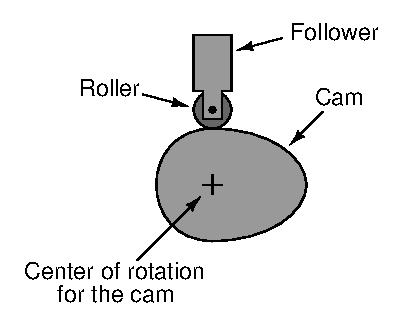
\includegraphics[width=15.5cm]{i01366x01.eps}$$

\vskip 20pt \vbox{\hrule \hbox{\strut \vrule{} {\bf Forslag til sokratisk diskusjon} \vrule} \hrule}

\begin{itemize}
\item{} En av de unike fordelene med å bruke kam i en ventilposisjoner er at kammen kan byttes ut med en annen {\it form}. Forklar hva endret kamform kan gjøre med oppførselen til en reguleringsventil.
\end{itemize}

\underbar{file i01366}
%(END_QUESTION)





%(BEGIN_ANSWER)

En {\it kam} er et roterende objekt med ujevn radius, som kan formes på ønsket måte for å gi en spesifikk sammenheng mellom vinkelutslag og lineær forskyvning:

$$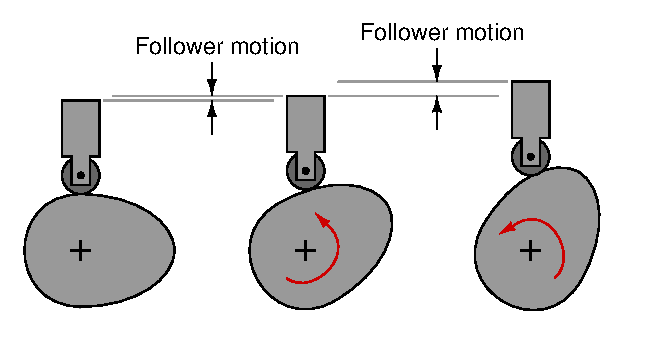
\includegraphics[width=15.5cm]{i01366x02.eps}$$

%(END_ANSWER)





%(BEGIN_NOTES)

Noen posisjonerere for lineære ventiler bruker leddmekanismer for å omsette lineær spindelbevegelse til roterende bevegelse, som deretter omdannes tilbake til lineær bevegelse gjennom en kam inne i posisjoneren. Nesten {\it alle} posisjonerere for roterende ventiler bruker kammer for å omsette den naturlige roterende spindelbevegelsen til lineær bevegelse inne i posisjoneren.

Studenter som kjenner motoroverhaling vil garantert vite hva en {\it kam} er, fordi toppventiler i stempelmotorer styres av kammer som roterer med halv veivakselhastighet. En motors {\it kamaksel} er en sammenhengende aksel med mange kammer, vanligvis én kam per ventil.

%INDEX% Final Control Elements, valve: positioner
%INDEX% Mechanics, cam: principle of

%(END_NOTES)

